\BiChapter{绪论}{introduction}
\BiSection{课题来源及研究的目的和意义}
x机器学习以及模式识别均属于人工智能范畴,机器学习源自于计算机科学,模式识别源自于工程学,尽管这两者源自于不同的背景,但这两者可以认为是同一个领域下的不同描述\citeup{PRML}。自计算机出生以来,人们一直都在探索一个问题:机器能否实现智能?早期的一部分研究人员试图从事物的机理出发,寻找模式背后的规律,比如在自然语言处理领域,最初人们从分析语法语义开始,企图让机器理解自然语言,并能实现一些类似于翻译之类的工作,但失败了,一个重要的原因是自然语言的规则错综复杂,要摸清其运作机理哪怕以目前的学科水平来看也几乎是难以实现的。

在随后的二三十年里,人类乐观地认为可以找到自然语言背后的运作机理,但实验结果都不尽人意,机理建模这条道路看起来像是一条死胡同。到了上世纪九十年代,统计机器学习开始成为主流,经过二十多年的高速发展,目前基于统计的建模方法成为了主流,而统计机器学习取得的成就远大于上世纪六十年到到九十年代取得的成果,当然这也不排除计算机运算能力的影响。

相比于机理建模,统计机器学习的出发点是从数据出发,建立一个可以刻画已有数据的概率分布,如果将机理建模比作是牛顿力学,那么统计学习就相当于统计力学。事实上,从统计的角度上去解决人工智能问题并不是一个新的想法,早在上世纪七十年代统计学习就已经开始出现。统计机器学习使我们不再需要研究模式背后的运作机理,并且通过它可以实现通用学习。如果说一个事物背后有一个函数决定了它的特性,那么我们不再需要研究这个函数究竟是什么形式,只要有足够多的数据,通过统计方法,选取恰当的模型,我们便可以在一定程度上拟合出这个函数,尽管我们拟合出的函数在大多数情况下都不等价于事物的本质函数,但如果它能在可允许的误差范围内正常工作,这就足够了。

统计机器学习方法的出现,使得工作重点转为寻找合适的模型上,事实上这也是统计机器学习其本质:经验风险最小化\citeup{MLbenzhi}。也就是说,我们应该如何寻找一个合适的模型,使得测试误差最小化?由于模型的选取取决于设计者的意愿,我们既可以选择一个简单的模型,比如线性函数,也可以选择一个复杂的函数,比如高次多项式函数,但是实际问题中,大多数情况下,如果使用简单的线性函数,数据在低维空间中是不可分的,为了使数据变得线性可分,我们可以将数据由低维空间映射到高维空间中,但这种方案引入了庞大的运算以至于计算机难以计算,我们称这种现象为“维数灾难”,即随着维数的线性增加,计算量指数地增大。又或者,我们一开始就不使用线性函数而使用较为复杂的函数比如高斯函数实现非线性分割,但由于我们不知道数据的分布形式,也难以将实际问题中的高维数据可视化,所以除非我们有关于数据分布的先验知识,否则并不知道我们选取的这个复杂的函数是否是合理的。

为了解决维数灾难,我们可以使用核函数,在低维空间中直接计算高维空间返回的结果,避开了高维空间的运算,这种方法也被称之为核方法,比如上世纪九十年代提出的支撑向量机(kernel-SVM)就是一种使用了核方法的分类器。而如果为了避免复杂函数的选取问题,我们可以使用神经网络。神经网络基于一种假说-----智能源自于单一的算法,在神经网络中,我们只需选取激活函数,即所谓的“单一的算法”,然后训练网络的连接权值,从而跳过函数选取步骤。

关于神经网络的表达能力方面,在理论上,柯尔莫格洛夫(Kolmogorov)证明了:只要给予足够多的神经元、合适的激活函数以及恰当的权值,任何从输入到输出的连续映射函数都可以用三层神经网络实现。如果从傅里叶理论上看,则相当于:任何连续函数都可以用足够多的谐波来逼近\citeup{Duda}。

柯尔莫格洛夫的定理说明了神经网络的表达能力与神经网络的层数无关,只与神经元的数目有关,似乎我们没有必要加深网络的深度,但Hastad与Goldmann在1991年提出了以下定理\citeup{learnForAI}

\begin{theorem}\label{theo:NNcomplexity}
为了计算一个函数$f_k \in \mathcal{F}_{k, N}$,深度为$k-1$的单调加权门限电路所需的规模至少为$2^{cN}$,其中常数$c>0$,$N>N_0$
\end{theorem}

由于神经网络与电路的联系十分密切,如果将定理\ref{theo:NNcomplexity} 转化为神经网络的术语,则为:深度为$k$的神经网络所能表达的函数,深度为$k-1$的神经网络为了达到同样的效果至少需要引入指数级规模的节点。

倘若从大脑科学的角度思考,我们已经知道,哺乳动物的大脑是一个深度结构,它可以将输入的模式在多个层次上进行抽象再表达,而每个层次对应着皮层的不同区域。以大脑在视觉系统上的工作机理为例,其工作过程依次经过如下几个步骤:边界检测、基本外形建立、逐渐地完善更为详尽外形\citeup{recognizeShape}。

在定理\ref{theo:NNcomplexity}以及大脑科学的启发下,我们对深度神经网络充满信心,因此神经网络研究人员花费数十年致力于深度神经网络的研究,然而直到2006年之前\citeup{Hinton2006, practicalGuide},我们都难以找到一个较好的算法来训练深度神经网络,其原因一方面是深度神经网络局部最优解繁多,导致深度神经网络比浅层神经网络更容易陷入局部最小值,另一方面则是受计算机运算能力的限制\citeup{diffcultyOfTrain}。

2006年Hinton提出了受限玻尔兹曼机以及深度置信网络的训练方法,通过贪婪逐层地训练\citeup{GreedyLayerWise},成功地实现了第一个深度神经网络,随后深度神经网络又发展处深度卷积网络、稀疏自动编码机\citeup{sparseRepres} 等方法,这些方法被统称为深度学习。目前,深度学习已应用到分类、回归、聚类、降维\citeup{reducingDimensionlity}、自然语言处理、信息检索、机器人学等任务中,且在某些领域中其应用效果已远远超越以前的机器学习方法。


\BiSection{国内外在该方向的研究现状及分析}
x2015年5月,Nature为纪念人工智能60周年开辟了"人工智能与机器人"专题,回顾了过去的研究历程与当今的研究热点,其中深度学习作为一个热点被加以介绍\citeup{nature2015}。目前深度学习在国内外都受到广泛关注,新的深度学习算法源源不断地被提出,在不久的将来,深度学习将会取得更多的成功。
\BiSubsection{神经网络与深度学习的发展状况}
x数十年来,神经网络研究人员在神经科学上付出了巨大心血,其研究之深入,范围之广,内容之繁杂是别的机器学习方法所难以企及的。我们今天看到的深度学习只是神经计算科学中的冰山一角,在它之下,是几十年探索积累起来的失败经验,这些模型中不乏观点新颖却无法工作的模型。这么多年来研究人员试图将神经网络理论化,然而到目前为止这项工作依然没有实现。
\BiSubsection{感知器时期}
x关于神经网络的想法由来已久,远在1800年人们已经开始研究神经网络,1943年心理学家Warren McCulloch与数理逻辑学Walter Pitts在总结前人关于神经工作原理的基础上将神经元工作数理化,随后冯·诺依曼在领导计算机设计时试图使用神经网络的形式而不是目前的指令形式\citeup{fengnuoyiman},限于当时科技水平限制最后并没有采用神经网络的方案。随着二十世纪六十年代控制论兴起以及计算机的出现,联接主义学者迫切地期待建立一个可用的神经网络数学模型,在这个环境中,受Warren McCulloch与Walter Pitts两人工作的启发下,Frank Rosenblatt提出了第一个神经元模型----感知器\citeup{overview},这标志着神经网络进入第一次浪潮。
\begin{figure}[!htbp]
\centering
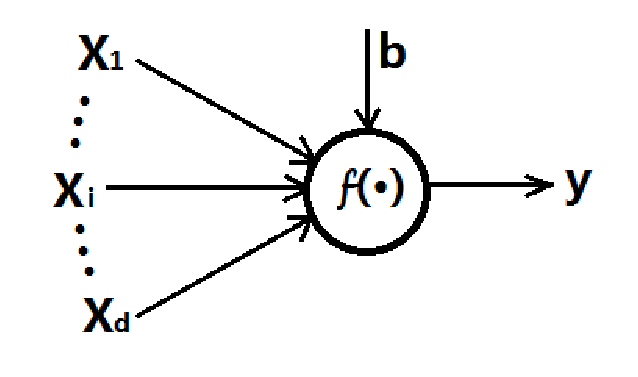
\includegraphics[width=0.33\textwidth]{NNnode.eps}
\caption{感知器模型}
\label{img:NNnode}
\end{figure}

如图\ref{img:NNnode} 所示,在感知器中,含有$d$个输入和1个输出,其中非线性激活函数为阶跃函数,即
\begin{equation}
y = \left\{
\begin{array}{cc}
1 & \text{~~~~若$\theta^Tx - b \geq 0$}\\
0 & \text{~~~~其他}\\
\end{array}
\right.
\end{equation}
式中$b$为偏置项,有时也称之为阈值。如果从神经科学的角度上解释,在感知器中,向量$x$相当于神经元接收到的刺激,而$\theta^T x$相当于刺激的叠加。当总的刺激量到达一定阈值$b$时,神经元被激活,即$y=1$,否则神经元对刺激不作反应,即$y=0$。

伴随感知器一同被提出的还包括感知器训练算法,其方法借鉴了生理学中关于反馈方面的思想,通过引入奖励与惩罚的概念,当某个训练样本被正确分类时,参数维持不变,若该样本被错误分类,则通过惩罚项对对参数进行更新\citeup{MLbenzhi}。

得益于非线性的激活函数,感知器网络可以实现逻辑功能以及非线性分类任务。例如,在输入维度为2的感知器网络中,若网络参数$\theta = [-2, -2]^T$,偏置$b = 3$,此时,这组参数构成的感知器即为门电路中的与非门。由于与非门可以构成与、或、非三种基本逻辑门,而这三者又可以构成所有的逻辑函数,因此我们有理由相信,恰当的感知器网络可以实现逻辑功能。事实上,六十年代感知器网络的提出,也确实解决了一些简单的人工智能任务。

神经网络第一次浪潮只持续了大约十年左右,究其原因,一方面,六十年代是电子计算机刚刚兴起的年代,人们更多地关注于计算机,导致感知器网络得不到重视,另一方面,限于电子管及早期晶体管的工艺,耗费大量的资源来建立一个感知器网络似乎也不太现实。此外,人们一直没有找到一种能较好地训练多层感知器网络的算法,导致了大批神经网络学者对其失去信心,因此,在六十年代末期,神经网络的研究进入第一个低谷。

\BiSubsection{反向传播时期}
x神经网络研究在八十年代进入第二次浪潮,最重要的原因是1986年Hinton、Remelhart和Williams等人提出了反向传播算法\citeup{bpalg},首次在手写数字识别任务上使用反向传播训练的神经网络,取得了较好的效果。此外,大规模集成电路的发展以及sigmoid等新的激活函数的应用也很大程度程度上推动了神经网络的发展。

反向传播算法通过链式求导,将偏导数从高层传送回低层,使得多层感知器网络中可以使用简单的梯度下降方法进行训练,尤其是在三层感知器网络中效果显著。随后,感知器网络也改名为神经网络,尽管如此,神经网络只是人为主观地对神经元建模,其本质与生物的神经系统是没有太大联系的,例如神经具有局部稀疏性而神经网络是非局部的,因此神经网络在生物学上被批评为缺乏真实性。

在这个时期,新的模型不断地被提出,比如使用Hebb规则全连接的反馈网络Hopfield网络\citeup{information}、将Hopfield网络随机化后的玻尔兹曼机\citeup{learnForBM}、具备模式变换不变性的卷积网络等\citeup{Duda},此外,一些新的技术例如快速传播、共轭梯度等也被应用到神经网络中。

九十年代人们开始尝试建立深度神经网络,但随着网络深度的加大,局部最优解增多,在参数没有被恰当地初始化的情况下,使用反向传播算法进行简单的梯度下降容易陷入局部极小值,人们难以找到一种较好的方法来训练深度网络。在硬件方面,九十年代计算机的计算能力仍不足以满足深度神经网络中大规模的运算。此外,同时期被提出的SVM方法可以在较少运算的前提下实现高性能的分类,因此,在九十年代中期,神经网络进入第二次低谷。

\BiSubsection{深度学习时期}
x深度神经网络的僵局一直持续到2006年,Hinton与Osindero在深度置信网络中使用一种无监督的逐层贪婪预训练受限玻尔兹曼机,使得权值被初始化到一个合适的位置,随后对整个网络使用全局的反向传播进行有监督的微调,在MNIST手写数字识别任务上超越了已有的记录\citeup{Hinton2006},随后,在受限玻尔兹曼机的基础上又发展出了稀疏编码与自动编码机等方法。深度置信网络是一种无监督学习,对应的,由LeCun等人提出的深度卷积网络实现了在深度结构下的有监督学习\citeup{lecun1989backpropagation,lecun1998gradient},成为第一个真正意义上的深度结构。

自2006年以来,深度学习的研究持续升温\citeup{frontierInAI,learnDeepModels},Google、Facebook、Microsoft等公司以及麻省理工、斯坦福大学、多伦多大学等高校投入大量资源到深度学习的相关研究中,麻省理工大学在2013年将深度学习评为十大突破技术的榜首\citeup{baidu}。由于深度学习需要训练样本容量足够大,而近年来大数据时代的到来,人们难以处理规模如此庞大的数据,所以某种程度上,深度学习与大数据是相辅相成的。

2012年前后,国内各大公司逐渐投入到深度学习相关的研究中,百度于2013年开展百度大脑计划,成立“深度学习研究院”,这是百度首次成立研究院,并于2014年邀请了深度学习的领军人物吴恩达作为首位院长。腾讯公司于2014年开发的Mariana平台将致力于研究深度学习在语音识别、图像识别和广告推荐上的应用。2015年京东将开展“JIMI”机器人项目,企图将深度学习应用到人工客服上。


\BiSection{深度学习在人工智能上的应用}
x深度学习在人工智能领域正在取得重大进展,利用这套技术解决了历史遗留的大量问题,目前已被应用到科学、商业、政策上。除了在传统的声、图、文领域深度学习掀起巨浪外,深度学习逐步开始渗入到生物学等其他领域。
\BiSubsection{语音识别}
x传统的语音识别一般使用混合高斯模型(GMM)或隐马尔可夫模型(HMM)\citeup{Duda},这些模型一般都比较简单,难以实现较高的正确率。Microsoft于2009年与Hinton在语音识别方面展开合作,并于2011年实现了深度学习在语音识别上的应用,该应用已经投入到WindowsPhone的语音识别“小娜”中。Google、百度也开展语音识别框架的改革,Google使用4$\sim$5层的神经网络,而百度使用9层的神经网络\citeup{baidu}。使用深度神经网络实现的语音识别在错误率上要比传统方法的错误率相对少$20\%\sim  30\%$左右。

\BiSubsection{图像识别}
x在声、图、文三个领域中,深度学习在图像识别上对识别效果的提升最显著。在MNIST手写数字识别任务中,使用传统识别方法的正确率一般为98\%左右,使用SVM能达到98.6\%的正确率,而使用深度学习方法在最好的情况下能达到99.79\%的正确率。在ImageNet1000任务中,对于1000个类别的识别,随着深度学习的研究进展,其识别效果分别经历了72\%、85\%、89\%、93\%等阶段,截止到2015年1月,由微软亚太研究院实现的最好效果为96.06\%\citeup{MS2015}。在SVHN街景门牌号的识别任务中,Google通过11层的神经网络对门牌号实现了97.84\%的正确率,这个系统已经帮助Google从街景中分析出全球近 1 亿个门牌号。

\BiSubsection{自然语言处理}
xMicrosoft于2012年在天津展示了使用深度学习训练的同声翻译系统,其英中翻译较传统方法更为流畅。然而,目前在自然语言处理领域,深度学习取得的效果并没有显著超越传统方法。相比于图像识别以及语音识别,自然语言处理一个难点在于上下文,尽管深度学习被认为是一种特征学习,但这种特征学习似乎并没有实现可以联系上下文的功能。自然语言处理在近期广受关注,深度学习研究人员认为下一个突破口将会出现在自然语言处理上。






